\documentclass[12pt]{article}
\usepackage[a4paper, left=2cm, right=2cm, top=2cm, bottom=2cm]{geometry}
\usepackage{dsfont}
\usepackage[fleqn]{amsmath}
\usepackage{amssymb,amstext}
\usepackage{graphicx}
\begin{document}
\setcounter{secnumdepth}{0}
\begin{center}
	UNIVERSIDADE FEDERAL DA PARAÍBA\\
	Cálculo II\\
	Terceira prova\\
	Paulo Ricardo Seganfredo Campana - 20210044220
\end{center}

\section{Questão 1.}
\subsection{i) $z=\arcsin(x-y), \quad x=s^{2}+t^{2}, \quad y=1-2st$}
\subsubsection{$\dfrac{\partial z}{\partial s}$}

\[\dfrac{\partial z}{\partial s} = \dfrac{\partial z}{\partial x} \dfrac{\partial x}{\partial s} + \dfrac{\partial z}{\partial y} \dfrac{\partial y}{\partial s} = \dfrac{1}{\sqrt{1-(x-y)^{2}}} \cdot 2s + \dfrac{1}{\sqrt{1-(x-y)^{2}}} \cdot (-1)(-2t) =\]
\[x-y = s^{2}+t^{2}+2st-1 = (s+t)^{2}-1\]
\[\dfrac{\partial z}{\partial s} = \dfrac{2s+2t}{\sqrt{1-((s+t)^{2}-1)^{2}}} \]
\[1-((s+t)^{2}-1)^{2} = 1-((s+t)^{4}+1-2(s+t)^{2}) =\]
\[-(s+t)^{4}+2(s+t)^{2} = (s+t)^{2}(2-(s+t)^{2})\]
\[\dfrac{\partial z}{\partial s} = \dfrac{2(s+t)}{\sqrt{(s+t)^{2}(2-(s+t)^{2})}} = \dfrac{2(s+t)}{(s+t)\sqrt{2-(s+t)^{2}}} = \dfrac{2}{\sqrt{2-(s+t)^{2}}}\]

\subsubsection{$\dfrac{\partial z}{\partial t}$}

\[\dfrac{\partial z}{\partial t} = \dfrac{\partial z}{\partial x} \dfrac{\partial x}{\partial t} + \dfrac{\partial z}{\partial y} \dfrac{\partial y}{\partial t} = \dfrac{1}{\sqrt{1-(x-y)^{2}}} \cdot 2t + \dfrac{1}{\sqrt{1-(x-y)^{2}}} \cdot (-1)(-2s)\]
\[\hspace{+19pt} = \dfrac{2}{\sqrt{2-(s+t)^{2}}}\]

\subsection{ii) $z=\tan \left( \dfrac{x}{y} \right), \quad x=2s+3t, \quad y=3s-2t$}
\subsubsection{$\dfrac{\partial z}{\partial s}$}

\[\dfrac{\partial z}{\partial s} = \dfrac{\partial z}{\partial x} \dfrac{\partial x}{\partial s} + \dfrac{\partial z}{\partial y} \dfrac{\partial y}{\partial s} = \sec^{2} \left( \dfrac{x}{y} \right) \cdot \dfrac{1}{y}\cdot 2 + \sec^{2} \left( \dfrac{x}{y} \right) \left( -\dfrac{1}{y^{2}} \right) \cdot x \cdot 3 = \sec^{2} \left( \dfrac{x}{y} \right) \left(\dfrac{2}{y} -\dfrac{3x}{y^{2}}\right)\]
\[\hspace{+19pt} = \sec^{2} \left( \dfrac{2s+3t}{3s-2t} \right) \left(\dfrac{2(3s-2t)-3(2s+3t)}{(3s-2t)^{2}}\right) = \sec^{2} \left( \dfrac{2s+3t}{3s-2t} \right) \left(\dfrac{-13t}{(3s-2t)^{2}}\right)\]

\subsubsection{$\dfrac{\partial z}{\partial t}$}

\[\dfrac{\partial z}{\partial t} = \dfrac{\partial z}{\partial x} \dfrac{\partial x}{\partial t} + \dfrac{\partial z}{\partial y} \dfrac{\partial y}{\partial t} = \sec^{2} \left( \dfrac{x}{y} \right) \cdot \dfrac{1}{y}\cdot 3 + \sec^{2} \left( \dfrac{x}{y} \right) \left( -\dfrac{1}{y^{2}} \right) \cdot x \cdot (-2) = \sec^{2} \left( \dfrac{x}{y} \right) \left(\dfrac{3}{y} +\dfrac{2x}{y^{2}}\right)\]
\[\hspace{+19pt} = \sec^{2} \left( \dfrac{2s+3t}{3s-2t} \right) \left(\dfrac{3(3s-2t)+2(2s+3t)}{(3s-2t)^{2}}\right) = \sec^{2} \left( \dfrac{2s+3t}{3s-2t} \right) \left(\dfrac{13s}{(3s-2t)^{2}}\right)\]

\section{Questão 2. $f(x,y) = 4x-3x^{3}-2xy^{2}$}
\subsection{i)}

\[\dfrac{\partial f}{\partial x} = 4-9x^{2}-2y^{2} = 0 \longrightarrow 9x^{2}+2y^{2}=4\]
\[\dfrac{\partial f}{\partial y} = -4xy = 0 \longrightarrow xy = 0 \longrightarrow x=0 \text{ ou } y=0\]
\[\text{se } x=0 \longrightarrow 2y^{2}=4 \longrightarrow y^{2}=2 \longrightarrow y = \pm \sqrt{2} \]
\[\text{se } y=0 \longrightarrow 9x^{2}=4 \longrightarrow x^{2}=\dfrac{9}{4} \longrightarrow x = \pm \dfrac{3}{2}\]

\subsection{ii)}

\[f_{xx} = -18x\]
\[f_{xy} = -4y \qquad D = \begin{vmatrix}
                          	-18x & -4y \\
                          	-4y & -4x
                          \end{vmatrix} \qquad detD = 72x^{2}-16y^{2}\]
\[f_{yy} = -4x\]

\[\text{em }(0,\pm \sqrt{2}), \quad detD < 0, \quad \text{ponto de sela}\]
\[\text{em }\left( \pm \dfrac{2}{3}, 0 \right), \ \  detD > 0\]
\[\text{para }\left( \dfrac{2}{3}, 0 \right), \quad\ \ f_{xx} < 0, \quad \text{ponto de máximo}\]
\[\text{para }\left( -\dfrac{2}{3}, 0 \right), \ \ \; f_{xx} > 0, \quad \text{ponto de mínimo}\]

\section{Questão 3. $f(x,y)=x+y-xy$}

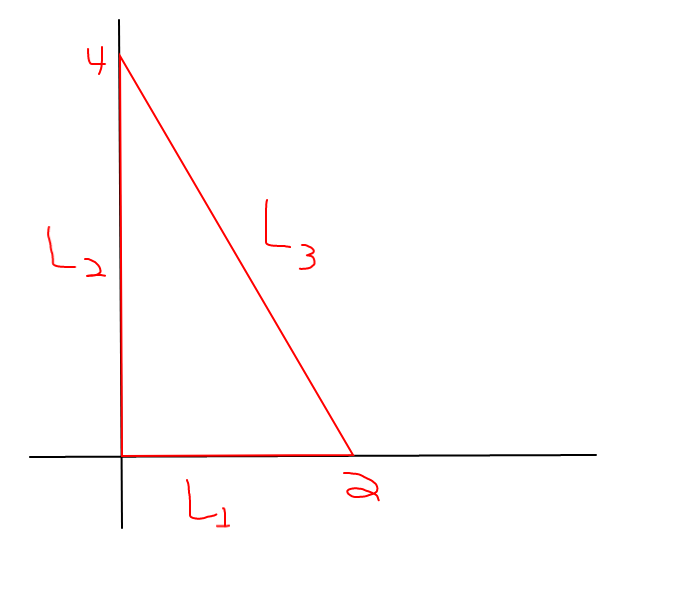
\includegraphics[scale = 0.4]{q2}

\[L_{1}: y=0, \quad 0 \leq x \leq 2, \quad f(x,0) = x\]
\[\hspace{+24pt} f(0,0) = 0\]
\[\hspace{+24pt} f(2,0) = 2\]
\[L_{2}: x=0, \quad 0 \leq y \leq 4, \quad f(0,y) = y\]
\[\hspace{+24pt} f(0,0) = 0\]
\[\hspace{+24pt} f(0,4) = 4\]
\[L_{3}: y = 4-2x, \quad f(x,4-2x) = x+4-2x-4x+2x^{2} = 2x^{2}-5x+4\]
\[\hspace{+24pt} \dfrac{d}{dx}(2x^{2}-5x+4) = 4x-5 = 0 \longrightarrow 4x = 5 \longrightarrow x = \dfrac{5}{4}\]
\[\hspace{+24pt} f \left( \dfrac{5}{4}, 4-\dfrac{10}{4} \right) = f \left( \dfrac{5}{4}, \dfrac{6}{4} \right) = \dfrac{5}{4} + \dfrac{6}{4} - \dfrac{30}{16} = \dfrac{7}{8}\]
\[(0,0) \text{ é ponto de mínimo}\]
\[(0,4) \text{ é ponto de máximo}\]

\section{Questão 4. $g(x,y,z) = y^{2}-xz=9$}

\[d^{2} = x^{2}+y^{2}+z^{2} = f(x,y,z)\]
\[\triangledown f = \lambda \triangledown g\]
\[\left\{\begin{array}{@{}l@{}}
	2x = \lambda(-z) \longrightarrow z = -\dfrac{2x}{\lambda}\\
	2y = \lambda2y \longrightarrow \lambda = 1\\
	2z = \lambda(-x) \longrightarrow 2\dfrac{-2x}{\lambda} = -x\lambda \longrightarrow -4x=-x\lambda^{2} \longrightarrow \lambda = \pm 2
\end{array} \right.\]

\[\text{para } \lambda = 2:\]
\[\left\{\begin{array}{@{}l@{}}
	2x = -2z \longrightarrow z = -x\\
	2y = 4y \longrightarrow y = 0 \\
	2z = -2x
\end{array} \right.\]
\[g(x,0,-x) = -x^{2} = 9, \quad x \notin \mathds{R}\]

\[\text{para } \lambda = -2:\]
\[\left\{\begin{array}{@{}l@{}}
	2x = 2z \longrightarrow z = x\\
	2y = 4y \longrightarrow y = 0 \\
	2z = 2x
\end{array} \right.\]
\[g(x,0,x) = x^{2} = 9, \quad x = \pm 3\]

\[\text{para } \lambda = 1:\]
\[\left\{\begin{array}{@{}l@{}}
	2x = -z \longrightarrow z = -2x\\
	2y = 2y \\
	2z = -x \longrightarrow -4x = -x \longrightarrow x=0, \quad z=0
\end{array} \right.\]
\[g(0,y,0) = y^{2}=9 \longrightarrow y = \pm 3\]

\[f(\pm3,0,\pm3) = 18\]
\[f(0,\pm 3,0) = 9\]
\[\text{portanto os pontos mais próximos a origem são }(0,3,0) \text{ e } (0,-3,0)\]

\section{Questão 5.}

\[f(x,y,z) = x^{2}+y^{2}+z^{2}\]
\[g(x,y,z) = x+2y+z=3\]
\[h(x,y,z) = x-y=4\]

\[\triangledown f = \lambda \triangledown g + \mu \triangledown h\]
\[\left\{\begin{array}{@{}l@{}}
	2x = \lambda + \mu \\
	2y = 2\lambda - \mu \\
	2z = \lambda
\end{array} \right. \longrightarrow \left\{\begin{array}{@{}l@{}}
	2x = 2z + \mu \\
	2y = 4z - \mu \longrightarrow 2x + 2y = 6z \longrightarrow x+y=3z \\
	\
\end{array} \right.\]
\[g(x,y,z) = x+2y+z = 3\]
\[\hspace{+60pt} 3z+y+z = 3\]
\[\hspace{+60pt} y = 3-4z\]
\[h(x,y,z) = x-y = 4\]
\[\hspace{+60pt} x-3+4z = 4\]
\[\hspace{+60pt} x = 7-4z\]
\[g(x,y,z) = x+2y+z = 3\]
\[\hspace{+60pt} 7-4z+6-8z+z = 3\]
\[\hspace{+60pt} -11z = -10\]
\[\hspace{+60pt} z = \dfrac{10}{11}\]
\[x = 7 - \dfrac{40}{11} = \dfrac{37}{11}\]
\[y = 3 - \dfrac{40}{11} = -\dfrac{7}{11}\]
\[\left( \dfrac{37}{11}, -\dfrac{7}{11}, \dfrac{10}{11} \right) \text{ é ponto de mínimo}\]
\\\\\\
$\dfrac{3}{4} \displaystyle \sum_{n=1}^{\infty} \dfrac{1}{16^{n}}$

\end{document}